\documentclass[a4paper,11pt]{article}
\usepackage{fullpage}
\usepackage{graphicx}
\usepackage{eqnarray,amsmath, amssymb}
\usepackage{bookmark}
\usepackage{hyperref}

\usepackage{listings}
\usepackage{changepage}

\makeatletter
\renewcommand\@seccntformat[1]{}
\makeatother
\hypersetup{pdfinfo={
Title = {ELEN3007-Assignment-2024},
Author = {Kgadile "Naar-Kie" Masemola},
CreationDate = {D:202409120836},
%ModDate = {D:202409040530},
Subject = {ELEN3XXX Paper Format, 2024}
%/Keywords (ELEN3007, naar_kie, paper, project)
}}

%%%%%%%%%%%%%%%%%%%%%%%%%%%%%%%%%%%%%%%%%%%%%%%%%%%%%%%%%%%%%%%%%%%%%%%%%%%%%%%%%%%%%%%%%%%%

\title{ELEN3007A Group \underline{27} - Assignment 2024: \\ 
\large \emph{Application of Bayes’ Theorem for Locating a Robot’s
Position in an Enclosed Area}}
\author{Kgadile E Masemola (876729)}
\date{September 13, 2024}

\begin{document}
\maketitle

\section{QUESTION 1:}  Why does $\theta_k$ not lie between $- \pi$ and $\pi$ for which $p(\theta_k | \alpha, \beta, B)$ would then be $\frac{1}{2\pi}$?

\subsection*{\underline{Solution 1:}}
The given setup of the problem says that the photodetectors are placed on the x-axis above which the robot is located. Therefore, the signal comes from one(top) side of the axis(horizontal in this case). This thus limits the range of the detectors to only capture collimated flashes within the azimuth $-\frac{\pi}{2}$ to $\frac{\pi}{2}$. . 

\section{QUESTION 2:}
Prove that
\begin{equation}
	p(x_k | \alpha, \beta, B) = \frac{\beta}{\pi (\beta^2 + (x_k - \alpha)^2)}
\end{equation}
\subsection*{\underline{Solution 2:}}
\label{sec:proof}
Using the relation $x_k = \alpha + \beta \tan \theta_k$ (given in the brief \cite{vanWyk2024}) and the prior PDF $p(\theta_k | \alpha, \beta, B) = f_{\Theta | \Lambda, \beta, B}(\cdot) = \frac{1}{\pi}$ and the transformation of random variables (notations for random variables defined \hyperref[sec:notation]{Solution 8}). The change of variables  $x = g(y) \Rightarrow \theta_k = g(x_k)$. The function $f(\theta)$ becomes $\tilde{f} = f(g(x))$. The given PDF $f_\Theta (\theta)$ corresponds to $f_X (x)$ with respect to new variable $x$. Therefore change of variables for PDF's equation adapted from \cite{bishop2006pattern} is:
\begin{equation}
	p_x(x) = p_\theta(\theta) \left| \frac{d\theta}{dx} \right| = p_\theta (g(x))|g^,(x)|
\end{equation}
using the correct notation and given $x_k$ relation:
\begin{align}
	f_X(x_k) &= f_\Theta (\theta_k) \times \left| \frac{d\theta_k}{dx_k} \right| = f_\Theta (\theta_k) \times \left| \left(\frac{dx_k}{d\theta_k} \right)^{-1} \right| \\
	&= \frac{1}{\pi} \times \left| \left( \frac{d}{d\theta_k}(\beta \tan \theta_k + \alpha) \right)^{-1}  \right| =\frac{1}{\pi} \times \left| \frac{1}{\beta \sec^2\theta_k} \right| \nonumber\\
	but \; \sec^2(\theta_k) &= 1 + \tan^2\theta_k \; and \; \tan\theta_k = \frac{x_k - \alpha}{\beta} \; (relation)\\
	so \; &= 1 + \left(\frac{x_k - \alpha}{\beta} \right)^2 = \frac{\beta^2 + (x_k - \alpha)^2}{\beta^2} \nonumber
\end{align}
	
\begin{align}
	\therefore \; f_X(x_k) &= \frac{1}{\pi} \times \frac{\beta^2}{\beta(\beta^2 + (x_k - \alpha)^2}\\
	and, \; so \; f_X(x_k) &\leftrightharpoons f_{X | \Lambda, \mathfrak{B}, B}(\, \cdot \, | \alpha, \beta) \; and \; f_\Theta (\theta_k) \leftrightharpoons f_{\Theta | \Lambda, \beta, B}(\cdot) \nonumber\\
	thus \; f_{X | \Lambda, \mathfrak{B}, B}(\, \cdot \, | \alpha, \beta) &= \frac{\beta}{\pi (\beta^2 + (x_k - \alpha)^2)} \; \blacksquare
\end{align}

\section{QUESTION 3:}
Plot $p(x_k | \alpha, \beta, B)$ and then relate its width at half maximum to the parameters of the PDF.

\subsection*{\underline{Solution 3:}}
The plot of the PDF $ p(x_k | \alpha, \beta, B) \Rightarrow f_{X | \Lambda, \mathfrak{B}, B}(x_k |\Lambda = \alpha, \mathfrak{B} = \beta)$ is shown in Figure 1 below. The \emph{parameters} are chosen to be $\alpha = 4; \beta = 2$ for $\{x_k \}^ {10} _{k = -10}$. It shows that the maximum value is when $x_k = 4 = \alpha$. At half maximum of \emph{these} paramaters, the width at half maximum of the distribution is $4 = 2 \beta$, half maximum height is $y = 0.1591536$.

\begin{figure}[h]
        \centering
        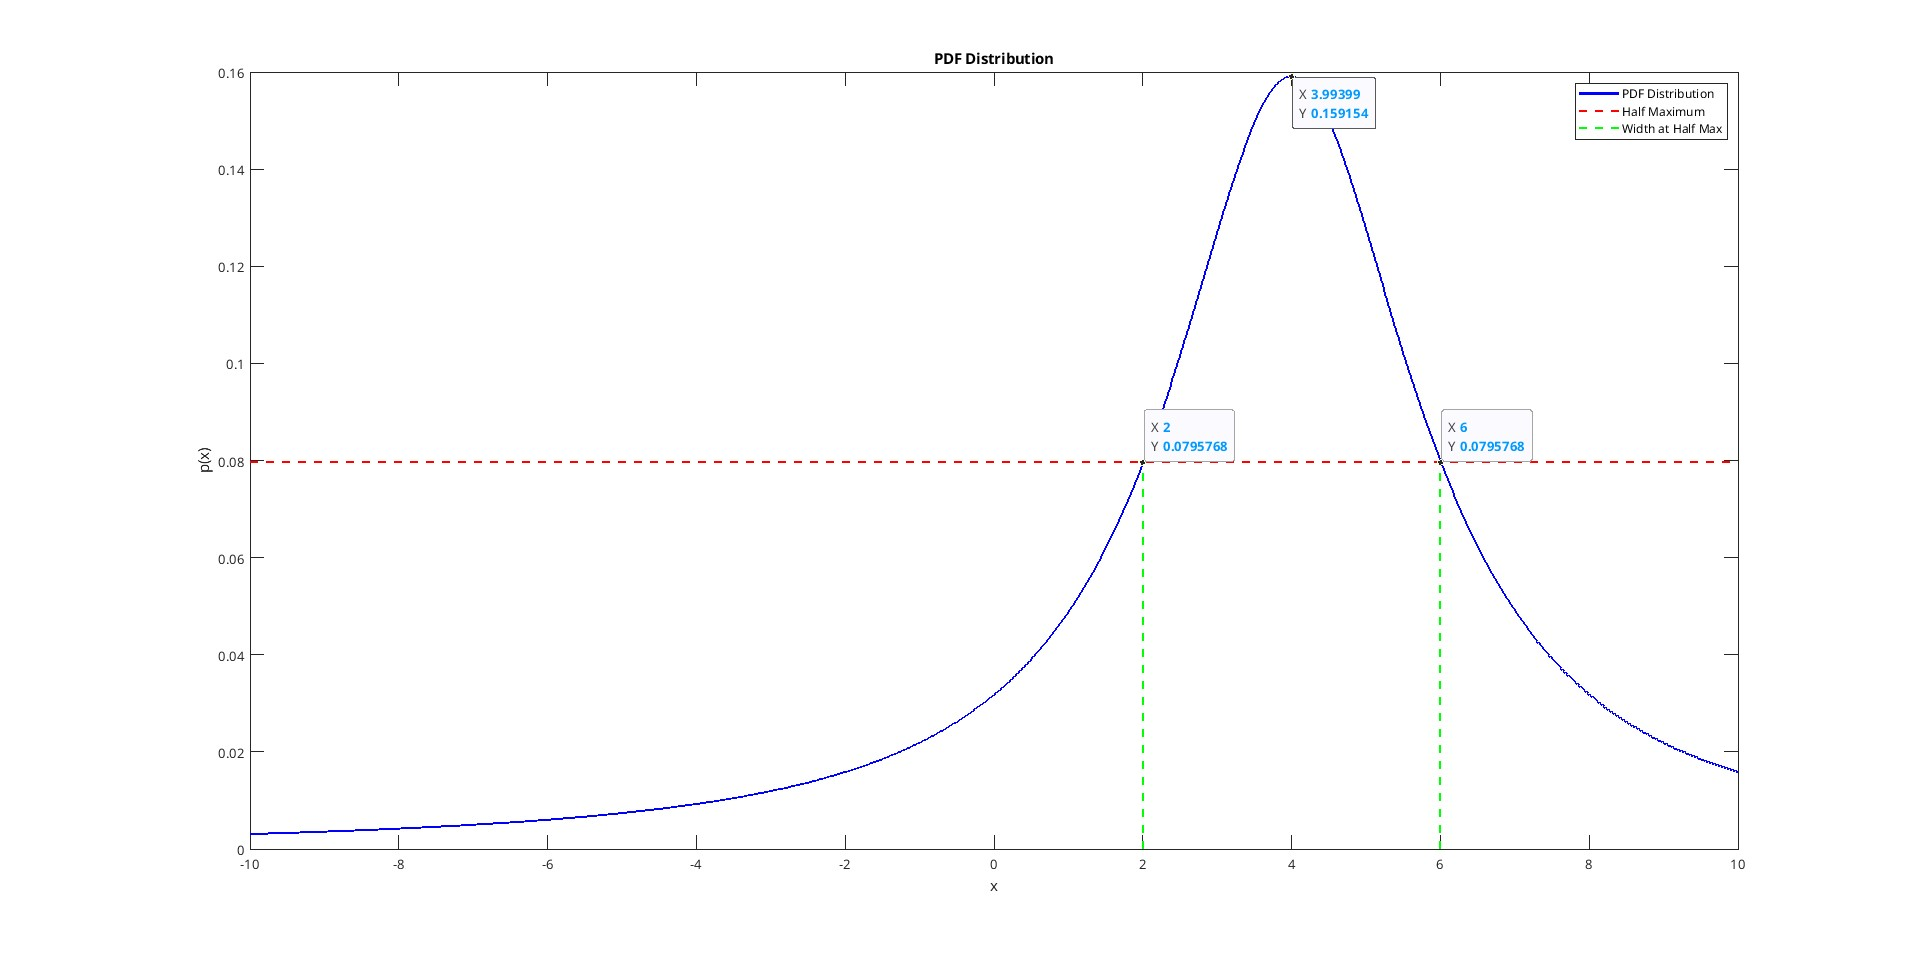
\includegraphics[scale=0.16]{q03pdfplot.jpg} 
        \caption{Q3 Plot of the PDF $p(x_k | \alpha, \beta, B)$}
\end{figure}


\section{QUESTION 4:}
Derive the expression for $p(\alpha | x_k, \beta, B)$.

\subsection*{\underline{Solution 4:}}
Bayes' Theorem requires: $p(\alpha | x_k, \beta, B) \Rightarrow f_{\Lambda | X, \mathfrak{B},B} (\, \cdot \, | x_k, \beta) = $. But, we can similarly use the same method as proof in \hyperref[sec:proof]{\textbf{Solution 2}}:

\section{QUESTION 5:}
Finally derive an expression for $p(\alpha | \{x_k\}^N _{k = 1}, \beta, B)$. (State all assumptions.)

\subsection*{\underline{Solution 5:}}
,

\section{QUESTION 6:}
Explain how one obtains the $x$-position of the robot from the result in (5.).

\subsection*{\underline{Solution 6:}}
The result in 5. can be used to obtain the position $x$-position of the robot by taking the product of the distributions of each $x_k$ measurement. This is due to the fact that the measurements are independent they are independent.\\
The $x$-position can also be obtained by locating the peak of the distribution (plot) and mapping it to the random variable variable axis. Additionally another method is to use Maximum-A-Posterior (MAP). We can also estimate the posterior mean by applying maximum likelyhood solution $\mu_{ML}$ to the mean of the data distribution and the mean of the prior distribution $\mu_0$. This way the estimate will be a compromise between $\mu_0$ and $\mu_{ML}$. The more measurements we use, the more the estimate approximate to $\mu_{ML}$.

\section{QUESTION 7:}
Implement the Bayesian position inference scheme in Matlab. Assume the robot is
located inside a confined square region of size $10$m $\times$ $10$m. Demonstrate your Bayes
estimator by inferring the robot’s $x$-position from the data/measurements $\{ x_k \}^{200} _{k = 1}$ in \emph{BayesData.mat}, with the robot’s $y$-position 4.5 m. Plot the Bayes posterior distribution for the first $N = 1, 2, 5$ and $30$ measurements. For this data, what is your best $x$-position estimate?

\subsection*{\underline{Solution 7:}}
,

\section{QUESTION 8:}
The notation presented above, deliberately does \emph{not} follow the conventions your Probs
lecturer introduced. Throughout your assignment, strictly use the notation prescribed for
use in Probs.
\subsection*{\underline{Solution 8:}}
\label{sec:notation}
Yes with the following Random Variable Notations and Equations: 
 	\begin{eqnarray}
		\Lambda (\cdot) = \alpha;\: \mathfrak{B}(\cdot) = \beta ; \: X(\cdot) = x_k; \: \Theta ( \cdot) = \theta_k \\		
		p(\theta_k | \alpha, \beta, B) = f_{\Theta | \Lambda, \beta, B}(\, \cdot \, | \alpha, \beta) = f_{\Theta | \Lambda, \beta, B}(\cdot)\\
		p(\alpha | x_k, \beta, B) = f_{\Lambda | X, \mathfrak{B}, B}(\, \cdot \, | x_k, \beta) = f_{\Lambda | X, \mathfrak{B}, B}(\cdot) \\\ 
		p(x_k |\alpha, \beta, B) = f_{X | \Lambda, \mathfrak{B}, B}(\, \cdot \, | \alpha, \beta)
	\end{eqnarray}

\section{QUESTION 9:}
Professional report with clear and effective data representation. The report must not have
a title page and is not allowed to exceed 5 pages in length.
\subsection*{\underline{Solution 9:}}
The report is presented in homework assignment form(statement and solution). Additionally, the following reference materials have been consulted for the assignment: \cite{leon2017probability}, \cite{bishop2006pattern}

\section{(Bonus) QUESTION 10:}
Infer both the $x$-position as well as the $y$-position of the robot. Estimate both $\alpha$ and $\beta$ for the PDF in Eq. (1).
\subsection*{Solution 10:}



\bibliographystyle{unsrt}
\bibliography{elen3007ref}

\newpage
\appendix

\makeatother
\section{Appendix A. - Matlab Inference Scheme Code}
\begin{lstlisting}
% Load the data
load('BayesData.mat');
\end{lstlisting}

\newpage
\section{Appendix B. - Matlab Scheme Plots}
	Plots


\end{document}
